\section{Anwendung}\raggedbottom 

Es sollen Karten in Videobildern erkannt werden. Dies soll über die Merkmale der Karten ermöglicht werden. Hierbei werden die Merkmale verwendet, die die Verfahren SIFT, SURF und ORB finden. Es soll verglichen werden, wie groß die Erkennungsrate für die Merkmale der einzelnen Verfahren ist.

Es wird ein Trainingsdatensatz erstellt, aus dem die Merkmale der einzelnen Karten berechnet werden.
Zudem wird ein Klassifikator vorgestellt, der mit Merkmalsabgleichen zwischen dem Bild einer unbekannten Karte und dem Trainingsdatensatz die unbekannte Karte klassifizieren kann.
Ein händisch erstellter Testdatensatz wird verwendet, um die Erkennungsrate des Klassifikators in Verbindung mit den von SIFT, SURF und ORB gefunden Merkmalen zu testen. Hierbei soll das beste Verfahren in Bezug auf Erkennungsrate und Geschwindigkeit gefunden werden.


\subsection{Aufbau einer Karte}

\begin{figure}[h]
    \centering
		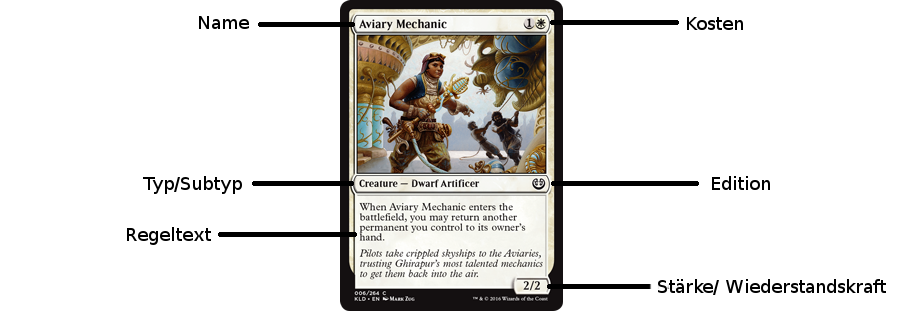
\includegraphics[scale=0.5]{bilder/sampleCard.png}
    	\caption{Beispielkarte ''Aviary Mechanic''}
    	\label{fig:sampleCard}
\end{figure}

Damit Karten identifiziert werden können, ist es wichtig den Aufbau einer Karte zu verstehen. So können Elemente gewählt werden, die geeignet sind, um Karten zu vergleichen.

Im Folgenden wird der Aufbau anhand der Karte in Abbildung \ref{fig:sampleCard} erklärt, ohne zu sehr auf die Regeln des Spieles einzugehen.

In der obersten Zeile der Karte findet sich der Kartenname  ''Aviary Mechanic'' und rechtsbünding die Kosten der Karte im Spiel. Der Name ist hierbei für jede Karte einzigartig, jedoch gibt es sehr viele andere Karten mit denselben Kosten.
Unter der Kopfzeile befindet sich das Kartenbild. Es ist einzigartig für eine Karte und wird später genutzt, um Karten in Videos zu erkennen.
Die Zeile unter dem Kartenbild beinhaltet den Typ 'Creature' und weitere Subtypen 'Dwarf Artificer' einer Karte und auf der rechten Seite ein Editionssymbol. Da es viele Karten mit dem gleichen Typ und aus der gleichen Edition gibt, sind diese auch nicht geeignet, um die Karte zu erkennen.
Unter dieser Zeile befindet sich ein großes Textfeld, welches den Regeltext der Karte beinhaltet.
Unten rechts befindet sich die ''Power'' und ''Toughness'' einer Kreatur. Da es viele Karten mit den gleichen Werten gibt, lässt sich diese Zahl auch nicht zum Erkennen nutzen.

Karten gehören im Spiel immer zu einer oder mehreren "Farben" (Weiß, Blau, Schwarz, Rot, Grün oder farblos). Der Kartenhintergrund entspricht jeweils dieser Farbe oder ist golden, wenn eine Karte zu mehren Farben gehört.
Jede Karte besitzt einen schwarzen Rand. Dieser wird später dafür verwendet Karten aus einem Spielbild zu lokaliseren. 

\subsubsection{Verwendbare Eigenschaften}

Von allen Elementen auf einer Karte sind nur Name und Bild in der Lage die Karte eindeutig zu indentifizieren. Der Name ist auf dem Videomaterial aufgrund der geringen Auflösung einer einzelnen Karten nicht lesbar.
Somit bleibt das Bild als einzige Möglichkeit, eine Karte aus einem Videobild eindeutig zu klassifizieren.


\subsection{Trainingsdatensatz}

Um Karten durch Merkmalsabgleiche zu erkennen, wird zuerst ein Datensatz an Karten benötigt, deren Klasse bekannt ist. Die Klasse ist in diesem Zusammenhang der Name der Karte. Über diesen Datensatz werden die Merkmale der einzelnen Karten berechnet, welche später mit den Merkmalen aus dem Testdatensatz verglichen werden.

\subsubsection{Aufbau}

Der Trainingsdatensatz besteht aus allen Karten der Edition ''Kaladesh'' und umfasst somit 264 Bilder. Jede Karte stellt eine eigene Klasse dar. Für jede Karte ist ein gelabeltes Bild vorhanden. Hierbei ist das Label der Name der Karte. Die Bilder haben alle eine Auflösung von $223 \times 311$ Pixeln.


\subsubsection{Erstellung}

Die Kartenbilder stammen von der offiziellen Seite von Wizards of the Coast. Jede Karte besitzt eine ID, mit welcher sich das Bild unter http://gatherer.wizards.com/Handlers/Image.ashx?multiverseid=ID\&type=card finden lässt.

Die Karten werden automatisch über ein Python Skript heruntergeladen. Dieses lädt zuerst für alle angegeben Editionen eine JSON Datei runter, die alle Informationen zu den Karten enthält. Aus dieser Datei werden die Karten IDs herausgelesen und über den oben genannten Link heruntergeladen und benannt.

\subsubsection{Vorverarbeitung}

Bevor mit SIFT, SURF und ORB die Features einer Karte aus dem Trainigsdatensatz gebildet werden, wird eine Vorverarbeitung durchgeführt, um später im Matching mit den Testdaten gute Ergebnisse zu erhalten.

Zuerst wird das Bild der Karte zugeschnitten, sodass nur noch der Bildbereich der Karte vorhanden ist. Dieser zugeschnittene Bereich ist $138 \times 188$ Pixel groß. Alle weiteren Operationen werden auf diesem Ausschnitt ausgeführt.
Das Bild wird auf eine Größe von $128 \times 128$ skaliert und in ein Graubild umgewandelt, da die drei Merkmalsverfahren mit Graubildern arbeiten.
In einem letzen Schritt wird das Bild noch mit einem $5 \times 5$ Gauß-Filter geglättet.

\subsection{Testdatensatz}

Der Testdatensatz besteht aus Bildern von Karten, die händisch aus Videos ausgeschnitten wurden. Die Karten stammen, so wie der Trainingsdatensatz, alle aus der Edition ''Kaladesh''. Er wird genutzt, um die Erkennungsrate der verschiedenen Verfahren beim Merkmalsabgleich zu bestimmen.

\subsubsection{Aufbau}
\label{sub:aufbau}

Der Testdatensatz besteht aus einem Grunddatensatz und drei aus diesem generierten Datensätzen.
Der Grunddatensatz besteht aus 300 benannten Bildern. Diese wurden per Hand aus Videobildern herausgeschnitten und klassifiziert. Die Bilder sind mit einer Auflösung von $85 \times 120$ Pixeln deutlich kleiner, als die Bilder des Trainingsdatensatzes.
Um die Größe des Datensatzes zu erhöhen und die Robustheit der Verfahren gegen häufig auftretende Bildveränderungen zu testen, wird der Datensatz künstlich erweitert.
Hierfür werden zwei Veränderungen betrachtet, die bei dem Videomaterial häufig auftreten.
Die eine ist die Rotation von Karten, die dadurch ensteht, dass Spieler die Karte bewegen und drehen. Die andere ist der Beleuchtungsunterschied, der durch verschiedene Aufnahmebedingungen ensteht. Hierbei werden diese Veränderungen für jede Karte 10 mal durchgeführt, damit die Ergebnisse nicht zu stark von der Zufälligkeit der Änderungen abhängt.

Diese Veränderungen werden sowohl einzeln, als auch in Kombination verwendet, sodass es am Ende 4 Datensätze gibt:

\begin{enumerate}
\item Grunddatensatz, 300 Bilder
\item Rotationsdatensatz, 3000 Bilder
\item Helligkeitdatensatz, 3000 Bilder
\item Rotation+Helligkeit Datensatz, 3000 Bilder
\end{enumerate}

Ein Beispiel für eine Karte in allen Datensätzen kann in Abbildung \ref{fig:testSet} gefunden werden.

\begin{figure}[h]
    \centering
		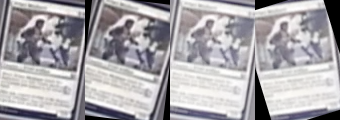
\includegraphics[scale=1.0]{bilder/testSet.png}
    	\caption{Von links nach rechts. Eine Karte aus dem Grunddatensatz. Die gleiche Karte im Rotationsdatensatz, die leicht gedreht wurde. Eine Karte aus dem Helligkeitsdatensatz, die künstlich aufgehellt wurde. Eine Karte aus dem Rotation+Helligkeit Datensatz, die sowohl gedreht als auch aufgehellt wurde.}
    	\label{fig:testSet}
\end{figure}

\subsubsection{Erstellung}

Die Rotation wird durch eine zufällige Drehung um $5°$ - $20°$ umgesetzt. Diese Rotation entspricht etwa der natürlichen Rotation die ensteht, wenn Spieler Karten nicht perfekt waagerecht legen.
Veränderungen in der Beleuchtung werden für jeden Pixel mit folgender Formel berechnet \footnote{\cite[S. 75]{Burg06}}:

\[
I'(x, y) = I(x, y)^\gamma
\]

Der Wert für $\gamma$ wird für jedes Bild zufällig zwischen 0.8 bis 1.8 gewählt. Die starke Tendenz zur Aufhellung anstatt Verdunklung ist dadruch bedründet, dass Spieler oft matte Hüllen um ihre Karten benutzen. Dieser matte Effekt lässt eine Karte deutlich heller erscheinen.
Diese Operationen werden auf jedes Bild im Grunddatensatz angewandt. Dadurch werden jeweils die anderen Datensätze erzeugt.

\subsubsection{Vorverarbeitung}

So wie beim Trainingsdatensatz wird auch für die Testbilder ein Vorverarbeitungsschritt durchgeführt, bevor die Bildmerkmale berechnet werden.
Das Bild wird zuerst auf eine Größe von $70 \times 85$ geschnitten, sodass nur die obere Hälfte der Karte zu sehen ist.
Das Bild wird in ein Graubild umgewandelt und auf eine Größe von $128 \times 128$ skaliert.

\subsection{Klassifikator}
\label{sec:klassifikator}

Im Folgenden wird ein Verfahren vorgestellt, mit dem einer Karte aus dem Testdansatz eine Klasse zugewiesen wird. 

\subsubsection{Idee}

Um einem Testbild eine Klasse zuzuweisen sollen die zuvor bestimmten Merkmale des Trainingsdatensatzes und die Merkmale des Testbildes genutzt werden.
Um diese Merkmale zu finden, werden SIFT, SURF und ORB benutzt.
Die Deskriptoren von SIFT, SURF und ORB sind so konstruiert, dass der gleiche oder ähnliche Bereich in einem Bild einen möglichst gleichen Deskriptorvektor ergibt. 
Dadurch sollten sich die Merkmale im Testbild in den Merkmalen des Trainigsdatensatz wiederfinden lassen.

Es wird der Raum betrachtet, in dem sich alle Vektoren aller Merkmale aus dem Trainingsdatensatz befinden. Nun wird für jedes Merkmal aus dem Testbild jeweils das Merkmal gefunden welches im Merkmalsraum, nach einer festgelegten Distanzfunktion, am nächsten ist.
Im Idealfall würde nun jedes Merkmal aus dem Testbild einem Merkmal der Klasse zugeordnet, zu der es wirklich gehört. Da sich die Trainings- und Testbilder jedoch so stark unterscheiden und die Merkmalsverfahren keine perfekten Ergebnisse liefern, werden einige Merkmale des Testbildes jedoch den falschen Klassen zugeordnet.
Um nun die richtige Klasse zu bestimmen, wird für jede Klasse eine Bewertung erstellt. Die Bewertungsfunktion soll sowohl viele übereinstimmende Merkmale belohnen als auch in Betracht ziehen, wie groß die Distanz zwischen den zugeordneten Merkmalen ist.


\subsubsection{Implementierung}

Im Folgenden wird für SIFT und SURF wird die euklidische Distanz als Distanzfunktionen genutzt. Da der Feature Vektor von ORB binär ist, wird für ORB die Hamming Distanz (siehe \ref{sub:hammingDistanz}) als Distanzfunktion genutzt.

Dadurch, dass jedes Merkmal des Testbildes einem Merkmale im Featureraum zugeordnet wurde, ergibt sich eine Menge $D_i$ für jede Klasse, die die Distanzen zwischen den Merkmalen enthält.
Die Bewertung $s_i$ für die Klasse $i$ wird definiert als: 

\[
s_i = \sum_{d \in D_i} \frac{1}{d^2}
\]

Die Bewertungsfunktion ist so gewählt, dass hohe Distanzen zwischen den Merkmalen weniger zu der Bewertung beitragen, als kleine Distanzen. Der Term $d^2$ bestraft große Distanzen, wodurch sehr gute Paare stärker in die Bewertung einfließen.

Nachdem alle Bewertungen $s_i$ berechnet wurden, wird das Testbild als die Karte klassifiziert, welche die höchste Bewertung hat.
Zudem wird aus allen Bewertungen bestimmt, wie sicher der Klassifikator ist, dass das Testbild richtig klassifiziert wurde.
Hierfür wird die sogenannte Softmax Funktion genutzt \footnote{\cite{Bishop:2006:PRM:1162264}}. Die Funktion nimmt einen Vektor an Werten und beschränkt alle Werte des Vektors in den Bereich [0, 1], sodas die Summe aller dieser neuen Werte 1 ist. Die Softmax Funktion ist definiert als:

\[
f_i(s) = \frac{e^{s_i}}{\sum_j e^j}
\]



\subsection{Durchführung}
\label{sub:durchführung}

Um die Erkennungsrate der verschiedenen Verfahren bewerten zu können, werden diese mit dem oben beschriebenen Klassifikator und den Testdatensätzen getestet.
Hierbei werden jeweils für SIFT, SURF und ORB die vier Testdatensätze durchlaufen und mit dem Klassifikator den Testbildern Klassen zugewiesen. 
Es wird festgehalten, welche Klasse den Testbildern mit welchem Softmaxwert zugewiesen wurde und ob diese Klasse die richige Klasse ist.
Desweiteren wird für jedes Verfahren gemessen, wie lange benötigt wird, um die Merkmale für die Testdaten zu bilden und diese zu klassifizieren. 
So kann im Weiteren ggf. eine Abwägung zwischen Geschwindigkeit und Erkennungsrate der Verfahren getroffen werden.

Die Ergebnisse werden in \ref{sec:auswertung} vorgestellt und ausgewertet.
